\section{A Letter from the Head}
Welcome to the School of Electrical and Computer Engineering (ECEN) at Oklahoma State University.

The School boasts 27 faculty members, including several IEEE Fellows and four recent and current NSF CAREER Award winners, along with approximately 300 undergraduate students and 150 graduate students pursuing the B.S., M.S. and Ph.D. degrees on both the Stillwater and Tulsa campuses. Students come to OSU from every state and approximately 120 countries making this a diverse, active, and exciting campus.

OSU offers a friendly and welcoming environment with easy access to faculty who are committed to excellence in the critical areas of teaching, scholarship and research. Our BS degree in Electrical Engineering is fully accredited by ABET. Your success as a student in ECEN is very important to us!

\begin{figure}
    \centering
    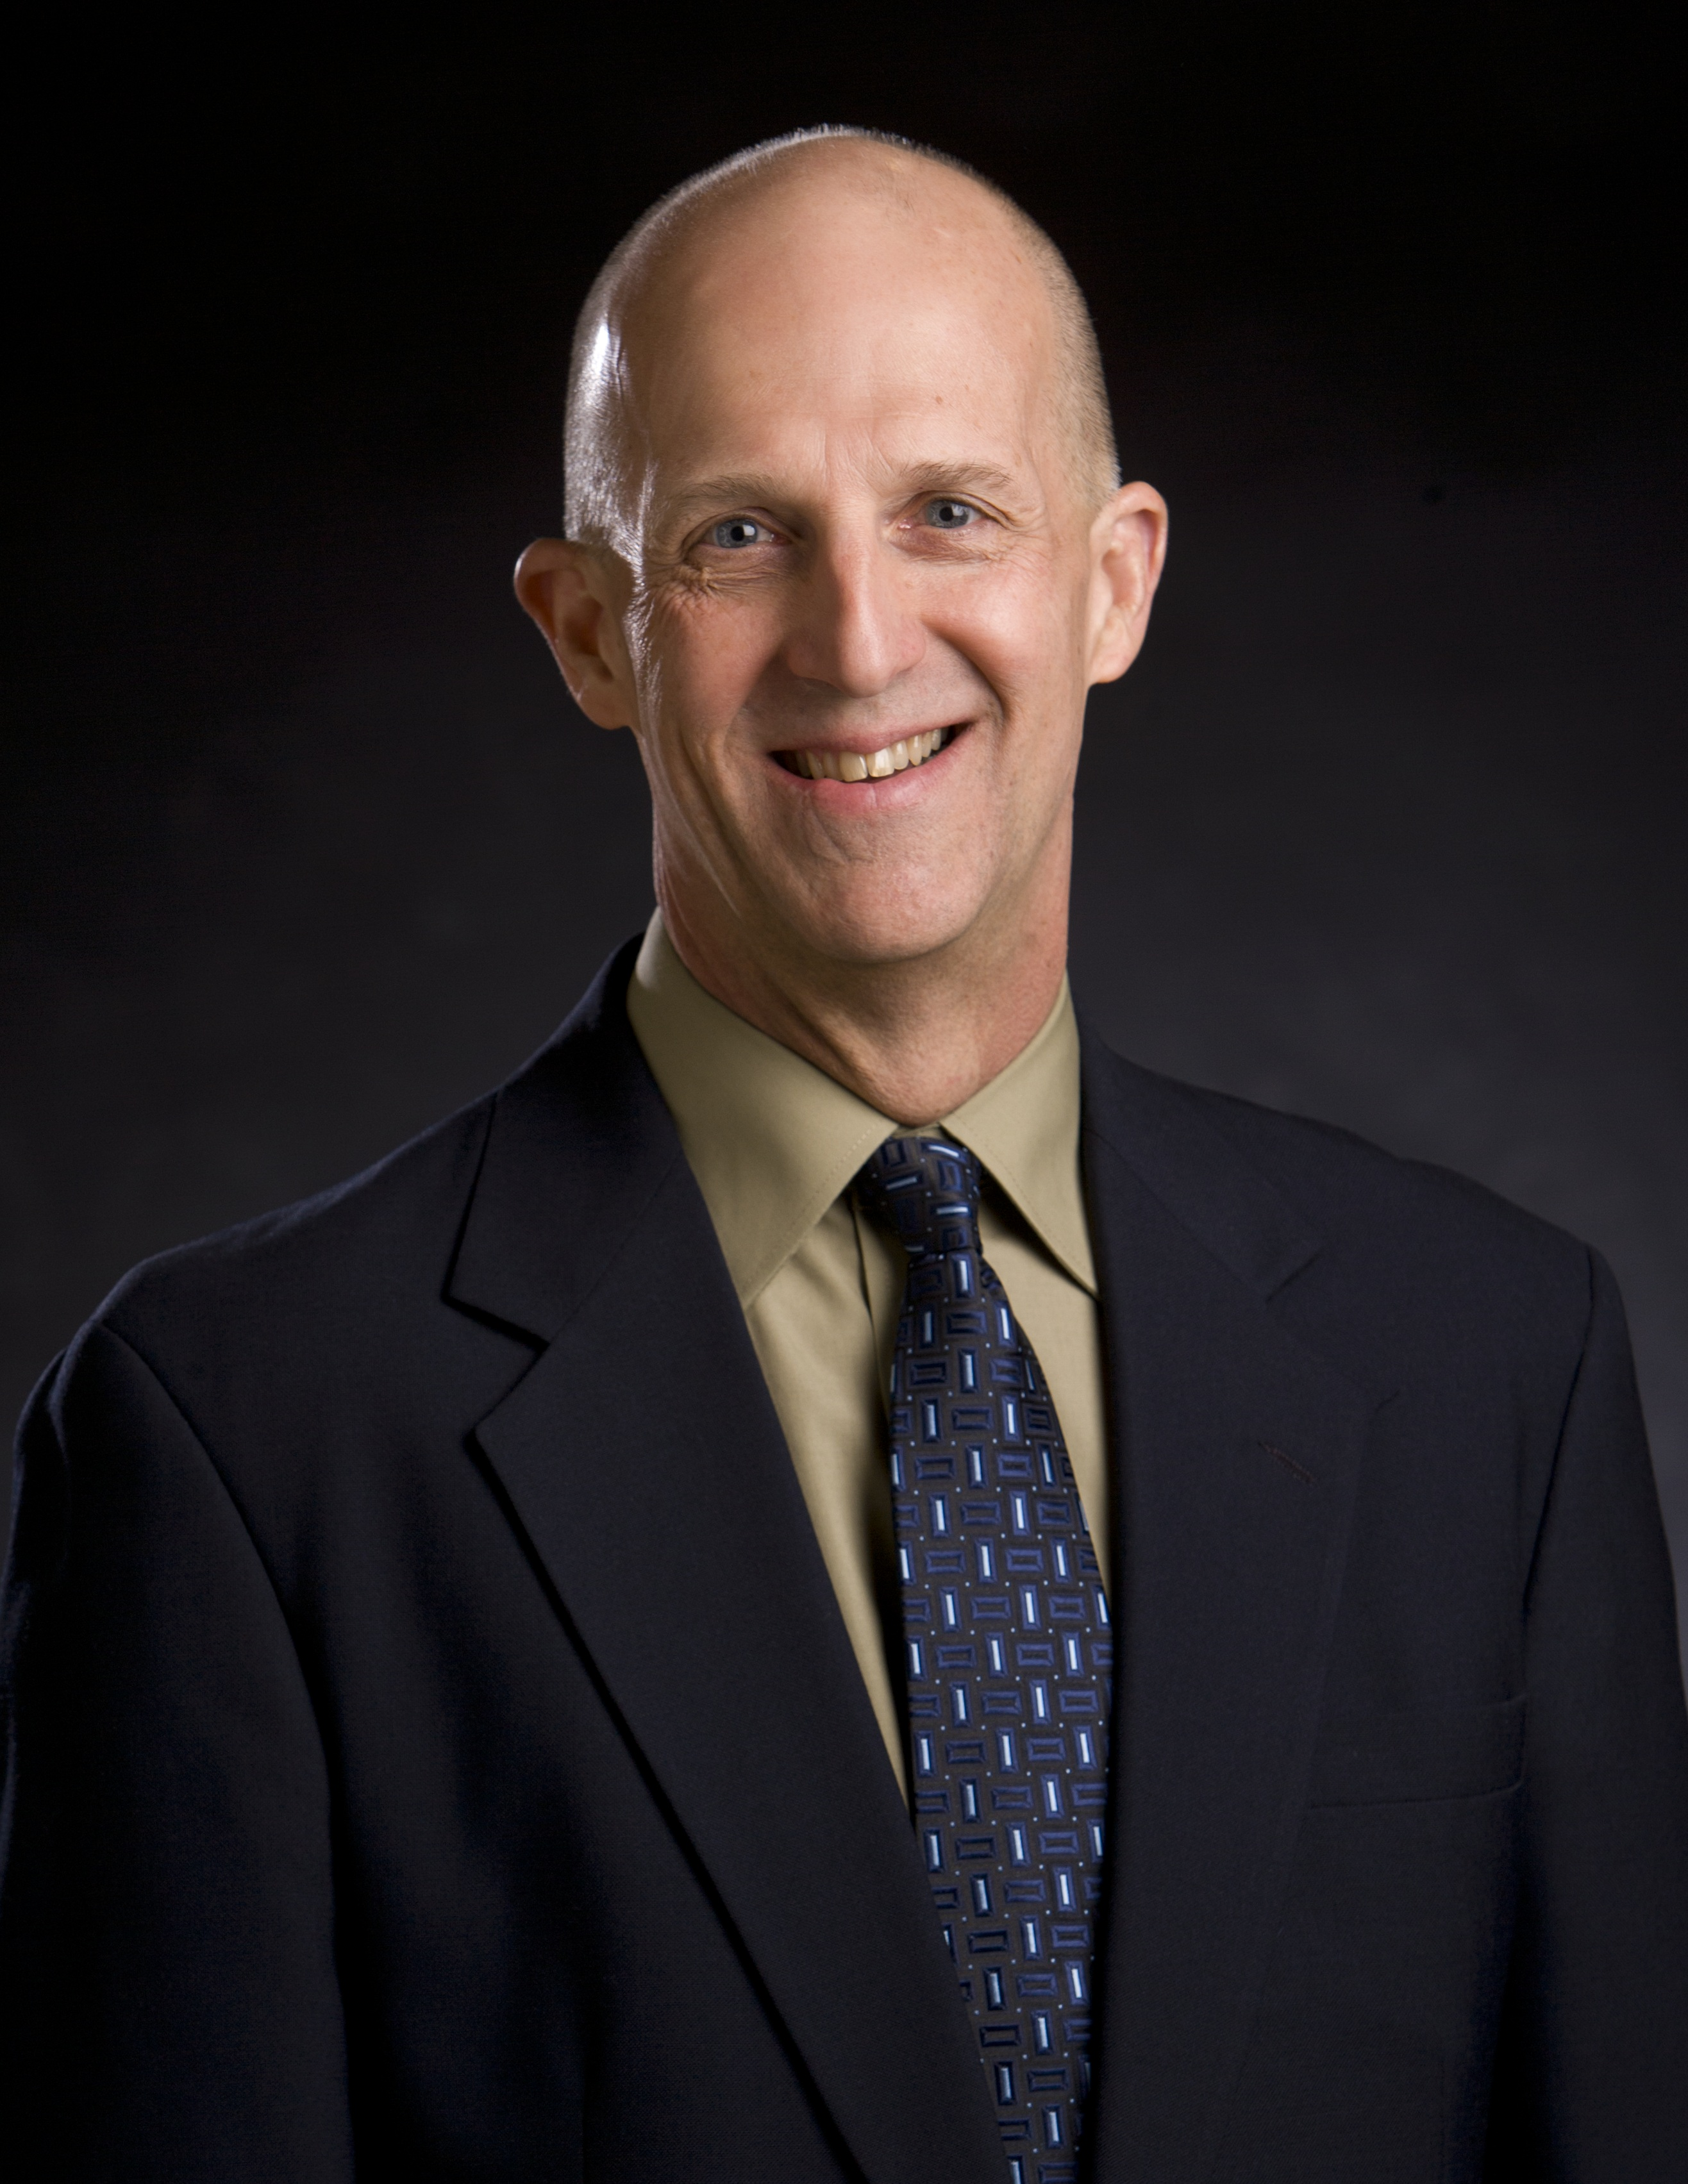
\includegraphics[width=0.25\columnwidth]{figs/DrTeague.jpg}
    \caption[Dr. Teague's Head]{Dr. Teague, Professor, Department Head}
\end{figure}
    

Over the past three years the School has experienced an unprecedented period of growth. We have been very fortunate to welcome nine new faculty members in the areas of computer engineering, communications, image processing and machine vision, biomedical engineering, and nanotechnology. We strive to emphasize excellence in all area of instruction, scholarship and research, as evidenced by a growing list of faculty and student accomplishments. Research and scholarly activities continue to expand, and thanks to an outstanding faculty annual research funding totals over $\$3.5$ million.

Our programs center around five primary thrust areas: communications, controls, and signal processing; computer engineering; lasers and photonics; electronics and mixed signal VLSI; and power. There are opportunities within these areas to accommodate the goals of almost any student interested in the various specializations within Electrical Engineering and Computer Engineering, as well as several interdisciplinary areas. We are especially excited about a new BS degree in Computer Engineering that we expect to introduce in 2008.

Excellent instruction and research laboratories are located in Engineering South and the Advanced Technology Research Center, a world-class facility located adjacent to Engineering South on the Stillwater campus. In Tulsa, the new Helmerich Advanced Technology Research Center houses a growing program in advanced materials and nanotechnology. 

Engineering graduates are in very high demand with over 170 companies actively recruiting at the most recent engineering career fair on campus. Our graduates are recognized as great employees who command high salaries. Our graduates are equally well prepared to study for an advanced degree, and many choose to pursue the M.S. or Ph.D. degree either at OSU or another outstanding university.

I’m very excited about our programs and what we have to offer. Please feel free to contact any faculty member or me for further information.

\subsection{ECE Mission Statement}

The School of Electrical and Computer Engineering – serving the needs of students, faculty, and those who employ our graduates – provides a comprehensive education in electrical or computer engineering. By providing both a breadth of knowledge and depth with design experience in selected areas, graduates are prepared to continue the lifelong process of education needed by active professionals in today's constantly changing global society.

